% !TEX root = main.tex
\section{Part 1: Identification of the boat  parameters}

In the assignment text we were given the following model of a ship:
\begin{subequations}
	\label{eq:completeModel}
		\begin{align}
				\dot{\xi_w} &= \psi_w \label{eq:xi_w}\\
				\dot{\psi_w} &= -\omega_0^2\xi_w-2\lambda\omega_0\psi_w+K_ww_w \label{eq:psi_w}\\
				\dot{\psi} &= r \label{eq:psi} \\
				\dot{r} &= -\frac{1}{T}r+\frac{K}{T}(\delta-b) \label{eq:r} \\
				\dot{b} &= w_b \label{eq:b} \\
				y &= \psi + \psi_w + v \label{eq:y}
		\end{align}
\end{subequations}

Where $\psi$ is the average heading, $\psi_w$ is a high frequency component due to the wave disturbance, $r$ the yaw rate and $b$ is a bias to the rudder angle $\delta$, $w_w$ and $w_b$ are white noice disturbances, $v$ is meassurement noise and $K$, $T$, $\lambda$ and $\omega_0$ are model parameters.


\subsection{1a)}

Using this model we can find the transfer function from $\delta$ to $\psi$. Taking the laplace transform of \cref{eq:psi} and \cref{eq:r} yields
\begin{subequations}
	\begin{align}
		s\psi &= r \label{eq:Lpsi}\\
		sr &= -\frac{1}{T}r + \frac{K}{T}(\delta-b) \label{eq:Lr}
	\end{align}
\end{subequations}

Assuming no disturbances $b = 0$ and combining \cref{eq:Lpsi} with \cref{eq:Lr} gives
\begin{equation}
	H_{ship}(s) = \frac{\psi}{\delta}(s) = \frac{K}{s^2T+s} \label{eq:H(s)}
\end{equation}

\subsection{1b)}

To find $K$ and $T$ we use the frequency response of \cref{eq:H(s)} with the frequencies $\omega_1 = 0.005\si{\radian\per\second}$ and $\omega_2 = 0.05\si{\radian\per\second}$, both with an amplitude of $1$. Using the provided ``ship'' we found the amplitudes experimentally (see \cref{fig:sin0.005} and \cref{fig:sin0.05}). This yields the equations
\begin{subequations}
	\begin{align}
		|H_{ship}(j\omega_1)| &= \frac{K}{\sqrt{T^2\omega_1^4 + \omega_1^2}} = 31.9787 \label{eq:omega_1}\\
		|H_{ship}(j\omega_2)| &= \frac{K}{\sqrt{T^2\omega_2^4 + \omega_2^2}} = 0.7847 \label{eq:omega_2}
	\end{align}
\end{subequations}

\begin{figure}
	\centering
	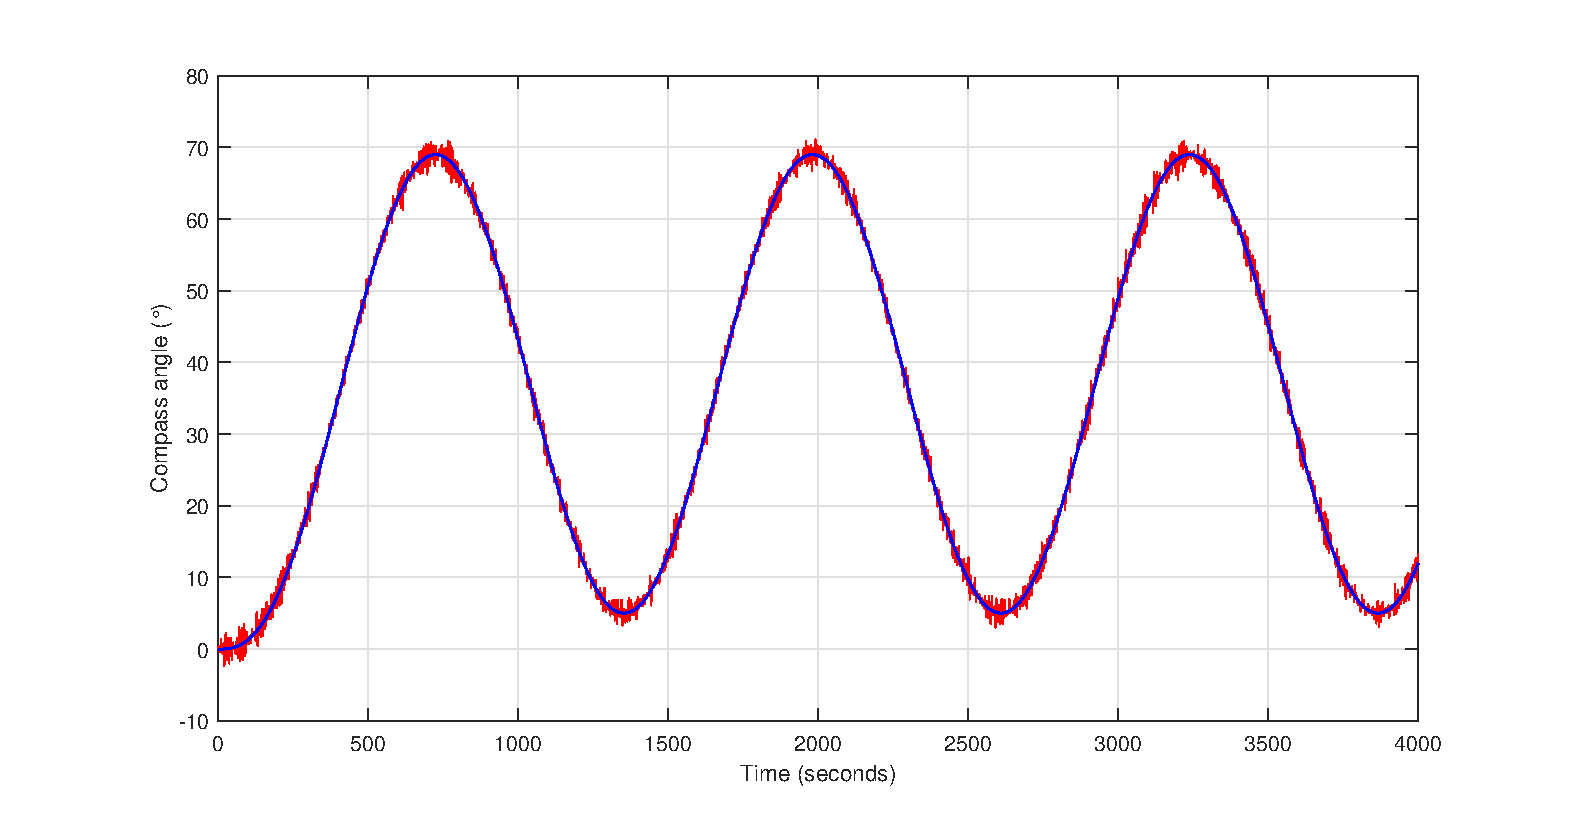
\includegraphics[width=\textwidth]{images/oppg1/sin0005.eps}
	\caption{Response of the ship given a input of \ensuremath{\sin{0.005}}.
		Blue line is without any noise, red line is with both waves and meassurement noise.}
	\label{fig:sin0.005}
\end{figure}

\begin{figure}
	\centering
	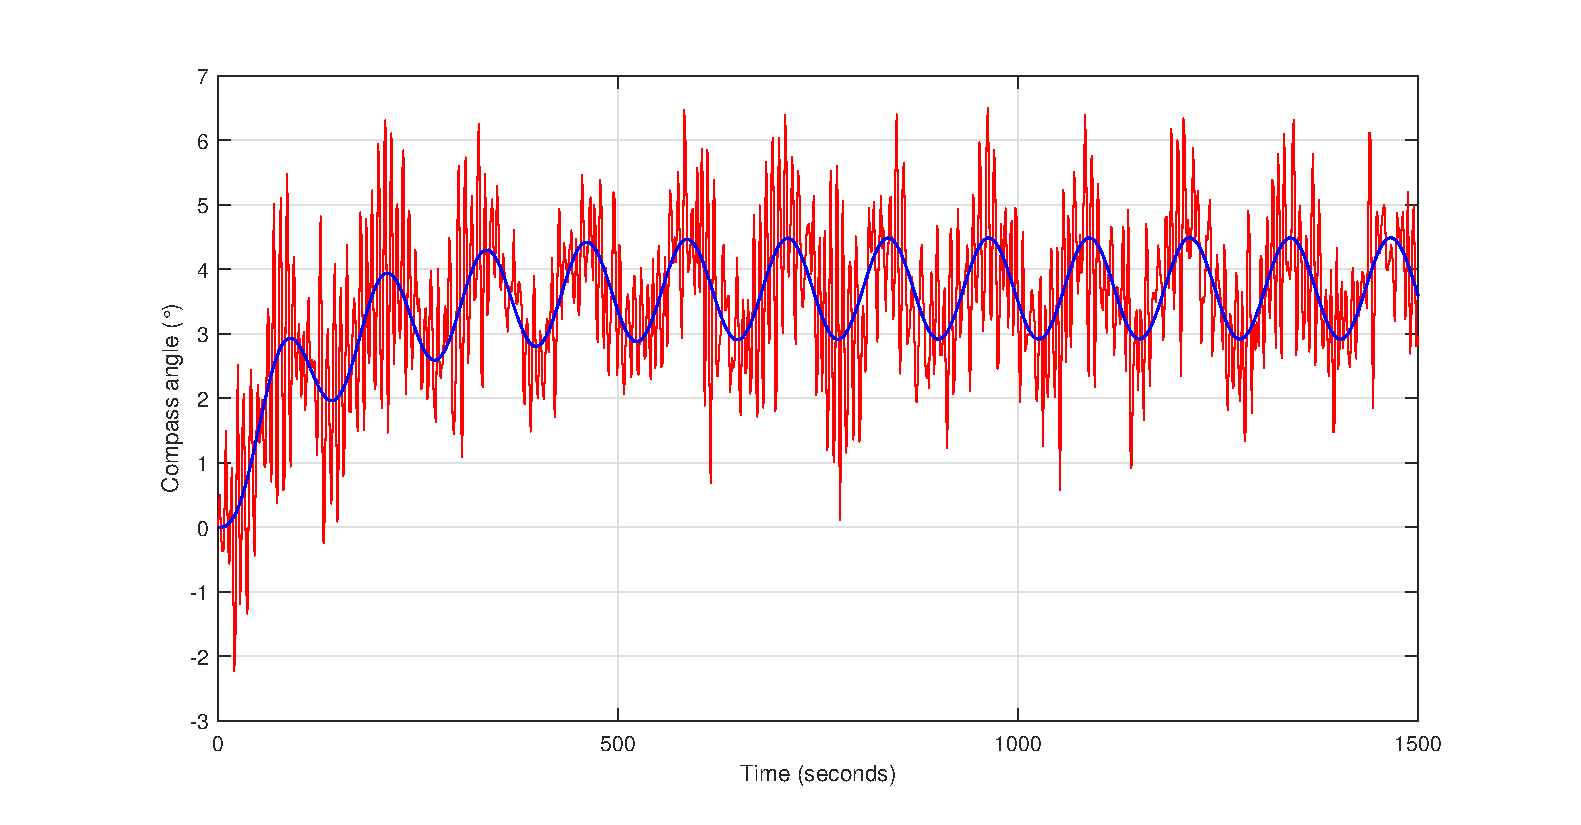
\includegraphics[width=\textwidth]{images/oppg1/sin005.eps}
	\caption{Response of the ship given a input of \ensuremath{\sin{0.05}}.
		Blue line is without any noise, red line is with both waves and meassurement noise.}
	\label{fig:sin0.05}
\end{figure}

Using Matlab function \texttt{solve} to solve this set of equations numerically yields
\begin{subequations}
	\begin{align}
		K &= 0.1742 \\
		T &= 86.5246
	\end{align}
\end{subequations}

\subsection{1c)}

If we simulate the ship with disturbance we see from \cref{fig:sin0.005}  and \cref{fig:sin0.05} that we get a noise component on top of the sinusoidal response. This makes it hard to find the true amplitude of the response, as we cannot simply use the half difference between the maximum and minimum.

\subsection{1d)}

If we apply a step input of $1$ degree at $t=0$ we get the response seen in \cref{fig:step_1}. As we can see the model is close to the ``actual'' ship at the beginning, but as the time increases, so does the errors of the model. This means that for small $t$s the model is a good approximation.

\begin{figure}
	\centering
	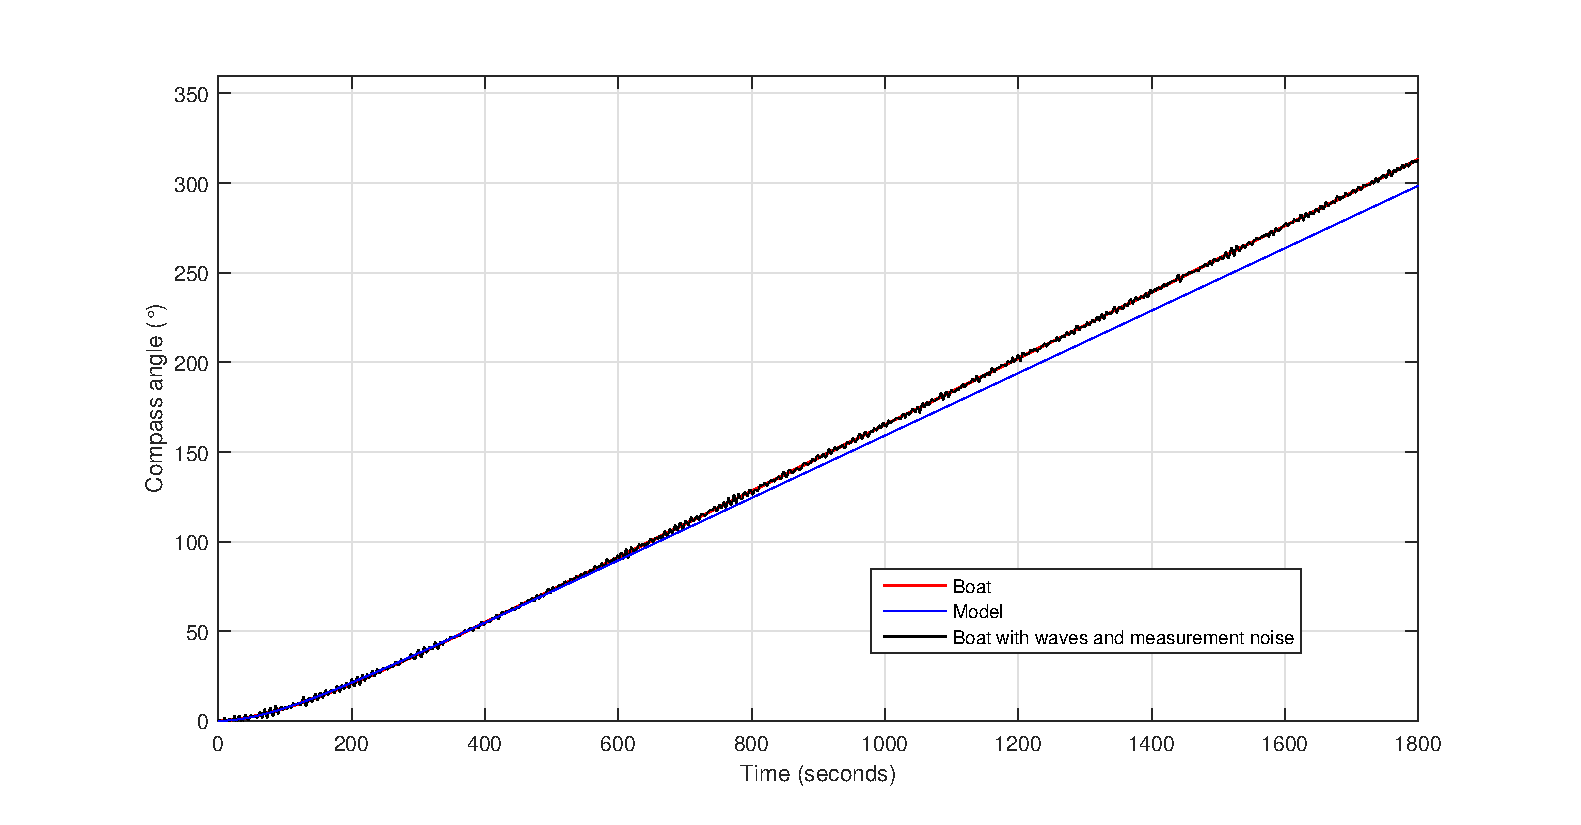
\includegraphics[width=\textwidth]{images/oppg1/step1_with_model_trafu.eps}
	\caption{Position of the ship and the model given a step input}
	\label{fig:step_1}
\end{figure}
